%%%%%%%%%%%%%%%%%%%%%%%%%%%%%%%%%%%%%%%%%%%%%%%%%%%%%%%%%%%%%%%%%%%%%%%%%%%
%
% Generic template for TFC/TFM/TFG/Tesis
%
% $Id: resultados.tex,v 1.7 2016/03/31 10:44:23 macias Exp $
%
% By:
%  + Javier Macías-Guarasa.
%    Departamento de Electrónica
%    Universidad de Alcalá
%  + Roberto Barra-Chicote.
%    Departamento de Ingeniería Electrónica
%    Universidad Politécnica de Madrid
% 
% Based on original sources by Roberto Barra, Manuel Ocaña, Jesús Nuevo, Pedro Revenga, Fernando Herránz and Noelia Hernández. Thanks a lot to all of them, and to the many anonymous contributors found (thanks to google) that provided help in setting all this up.
%
% See also the additionalContributors.txt file to check the name of additional contributors to this work.
%
% If you think you can add pieces of relevant/useful examples, improvements, please contact us at (macias@depeca.uah.es)
%
% You can freely use this template and please contribute with comments or suggestions!!!
%
%%%%%%%%%%%%%%%%%%%%%%%%%%%%%%%%%%%%%%%%%%%%%%%%%%%%%%%%%%%%%%%%%%%%%%%%%%%

\chapter{Evaluación y resultados}\label{cha:resultados}

Una vez realizados todos los pasos indicados en el Capítulo~\ref{cha:desarrollo}, se debe llevar a cabo la comprobación y medición de rendimiento de los algoritmos.
En este capítulo, se explicará la realización de pruebas de comprobación de funcionamiento de los algoritmos y, posteriormente, las mediciones llevadas a cabo para conocer el rendimiento de los mismos.

\section{Pruebas unitarias de comprobación}\label{sec:unitarias}



\section{Medidas de ejecución}\label{sec:medidas}

Para poder medir el rendimiento de los algoritmos, se han tenido en cuenta varios factores.
Estos factores son el tamaño del \textit{software} resultante, la energía consumida durante la ejecución del algoritmo y el tiempo de ejecución del algoritmo.

\subsection{Consumo energético}\label{subsec:energia}

Para realizar la medición del consumo energético, se ha empleado el dispositivos INA219~\cite{ina219}.
Este dispositivo se empleará junto a una tarjeta ESP32, de forma que el dispositivo INA219 realiza las medidas de energía consumida y el dispositivo ESP32 envía estos datos al ordenador conectado.


\subsection{Tiempo de ejecución}\label{subsec:tiempo}

En cuanto al tiempo de ejecución se refiere, para poder conseguir una medida significativa, se ha realizado la ejecución de cada función que componen los algoritmos.
Para ello, se obtendrá una medida del tiempo transcurrido al inicio de la función y otra al finalizar esta, de forma que la resta de ambas suponga el tiempo requerido para la ejecución de esta función.


\subsubsection{Temporización en dispositivo ESP32}\label{subsubsec:esp32_temp}

Para poder medir el tiempo transcurrido durante la ejecución de cada función del algoritmo es necesaria la inclusión de la librería \texttt{esp\_timer.h} y la utilización de la función \texttt{esp\_timer\_get\_time}~\cite{esp_timer_get_time}.
Se ha hecho uso de esta función ya que aporta una precisión del orden de microsegundos a la hora de llevar a cabo la medición de tiempo.
La medición se realiza mediante el Código~\ref{lst:esp_timer_get_time}.
En este código, la variable \texttt{time\_ini} representa el tiempo transcurrido al inicio de la función, \texttt{time\_end} indica el tiempo transcurrido hasta el final de la función y \texttt{time\_ref} se utiliza para obtener el tiempo transcurrido en la llamada a la obtención del tiempo transcurrido.
Con esto, el tiempo necesario para la ejecución de la función (en el Código~\ref{lst:esp_timer_get_time} la función medida es la generación de claves) se obtendría mediante la resta del tiempo al finalizar la ejecución de la función menos el tiempo de inicio y el tiempo requerido para la obtención del tiempo transcurrido.
Es decir, $tiempo_{funcion} = tiempo_{final} - tiempo_{inicio} - (tiempo_{referencia} - tiempo_{final})$.

\begin{lstlisting}[label={lst:esp_timer_get_time},style=Bashnice,firstnumber=1,caption={Medición temporal en el dispositivo ESP32.}]
time_ini = esp_timer_get_time();
crypto_sign_keypair(pk, sk);
time_end = esp_timer_get_time();
time_ref = esp_timer_get_time();
\end{lstlisting}


\subsubsection{Temporización en dispositivo RP2040}\label{subsubsec:rp2040_temp}

Para llevar a cabo la medición del tiempo transcurrido en el dispositivo RP2040 es necesaria la inclusión de la librería \texttt{pico/time.h} y la utilización de la función \texttt{get\_absolute\_time}~\cite{get_absolute_time}.
Se ha escogido esta función ya que otorga una precisión de microsegundos.
La medición del tiempo transcurrido se ha realizado, mediante el Código~\ref{lst:get_absolute_time}.
Para este caso, las variables utilizadas implican el mismo funcionamiento que en el caso del dispositivo ESP32, mostrado en la Subsección~\ref{subsubsec:esp32_temp}.
Por ello, la forma de obtener el tiempo necesario para la ejecución de la función es, también, idéntica al caso del dispositivo ESP32.

\begin{lstlisting}[label={lst:get_absolute_time},style=Bashnice,firstnumber=1,caption={Medición temporal en el dispositivo RP2040.}]
time_ini = get_absolute_time();
crypto_kem_keypair(pk, sk);
time_end = get_absolute_time();
time_ref = get_absolute_time();
\end{lstlisting}

\subsubsection{Temporización en dispositivo STM32}\label{subsubsec:stm32_temp}

En cuanto a la medición del tiempo transcurrido en el dispositivo STM32 es necesario llevar a cabo la diferenciación entre McEliece348864 y los algoritmos incluidos en el repositorio PQM4.
Para el primero, debido a la gran cantidad de memoria requerida para el algoritmo y su ejecución, no es viable la posibilidad de incluir algún módulo de comunicación entre un ordenador y el dispositivo.
Por ello, el único método utilizable consiste en el iluminado y apagado de los LEDs que incluye el dispositivo a modo de indicador de inicio y final de ejecución.

En el caso de los algoritmos incluidos en el repositorio PQM4, la ejecución de estos nos aporta el número de ciclos requeridos para su ejecución.

Para todos aquellos algoritmos que requieran de un mensaje para firmar, se utilizará el mensaje \textit{Esto es una prueba de la firma de mensajes utilizando (nombre del algoritmo).}.

\subsection{Pruebas en dispositivo ESP32}\label{subsec:esp32_res}

Para la medición de la temporización de los algoritmos Dilithium y Kyber, se ha llevado a cabo la ejecución de las 3 funciones características del algoritmo un total de 1000 iteraciones.
Esta prueba requiere de la eliminación del módulo \textit{watchdog} del sistema operativo utilizado por el dispositivo ESP32.
Una vez se han realizado todas las ejecuciones, se ha obtenido el tiempo medio de ejecución y se ha representado en los gráficos mostrados en Figura~\ref{fig:dilihtium_res} y la Figura~\ref{fig:kyber_res}.

\begin{figure}[h]
    \centering
    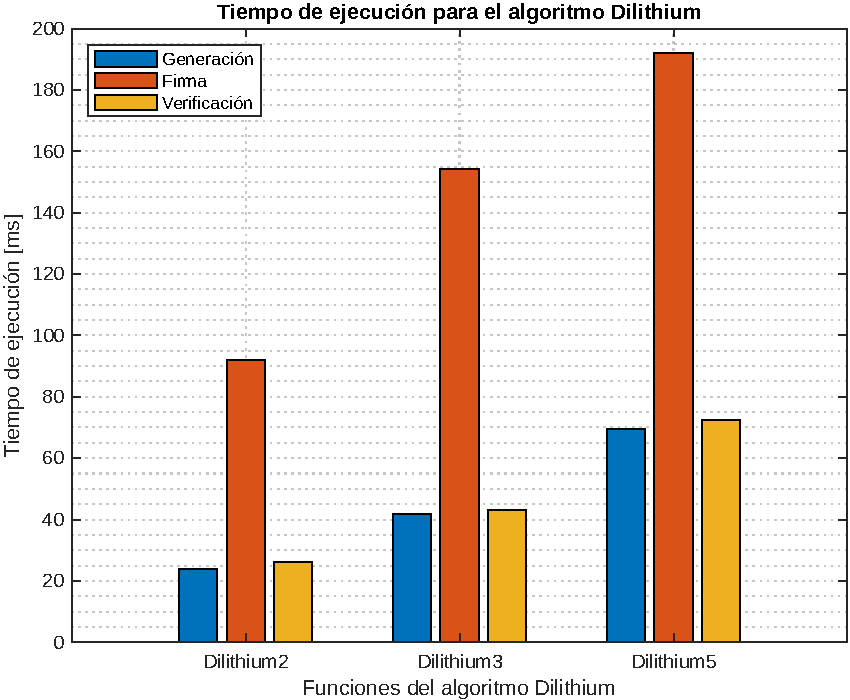
\includegraphics[width=0.6\textwidth]{figures/Dilithium.pdf}
    \caption{Tiempo de ejecución medio para el algoritmo Dilithium.}
    \label{fig:dilihtium_res}
\end{figure}

Respecto a la ejecución del algoritmo Dilithium, se observa que el tiempo requerido para la verificación de la firma es ligeramente superior al requerido para la generación de las claves, mientras que el tiempo requerido para la firma de un mensaje es entre X y X veces superior al requerido para la generación de las claves. %//TODO: cambiar las X
Es importante mencionar que, en el caso de la firma de un mensaje, el tiempo puede variar notablemente entre ejecuciones.
Por ejemplo, en la versión Dilithium2, el tiempo mínimo observado ha sido %//TODO: indicar mínimos y máximos

\begin{figure}[h]
    \centering
    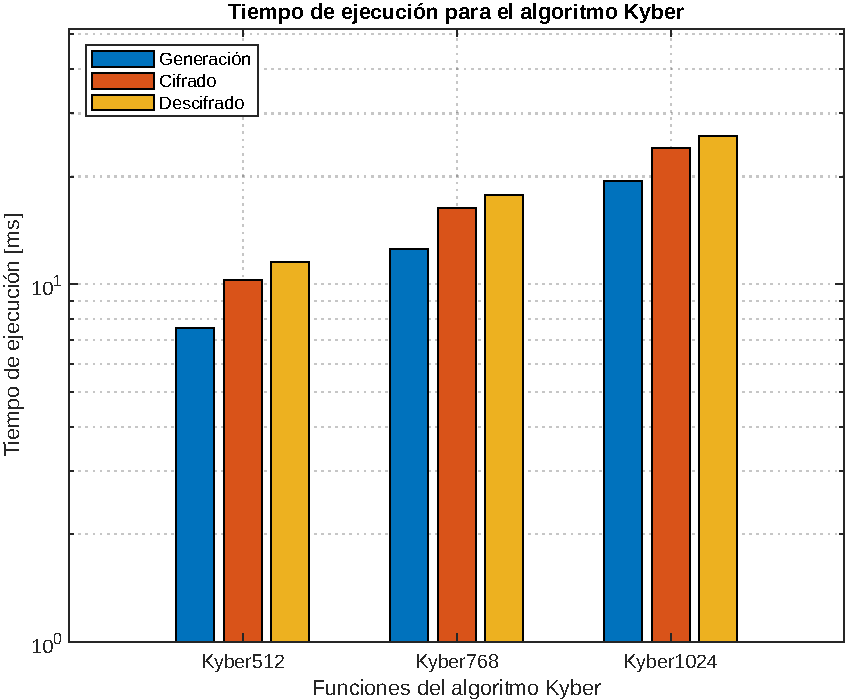
\includegraphics[width=0.6\textwidth]{figures/Kyber.pdf}
    \caption{Tiempo de ejecución medio para el algoritmo Kyber.}
    \label{fig:kyber_res}
\end{figure}

En el caso del algoritmo Kyber, los tiempos requeridos para las 3 funciones son más cercanos entre sí, como se puede comprobar en la Figura~\ref{fig:kyber_res}.


\subsection{Pruebas en dispositivo RP2040}\label{subsec:rp2040_res}


\begin{figure}[h]
    \centering
    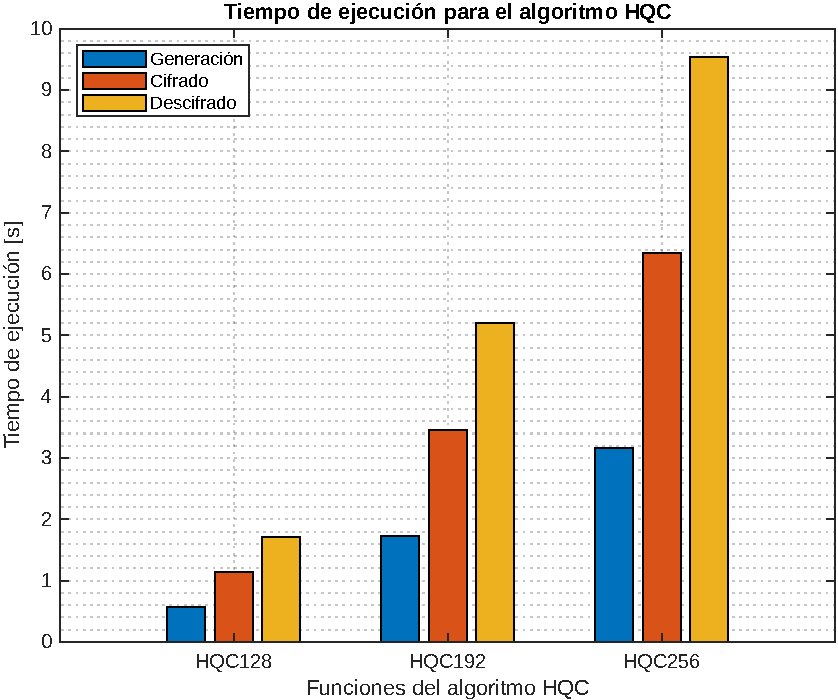
\includegraphics[width=0.6\textwidth]{figures/HQC.pdf}
    \caption{Tiempo de ejecución medio para el algoritmo HQC.}
    \label{fig:hqc_res}
\end{figure}


\subsection{Pruebas en dispositivo STM32}\label{subsec:stm32_res}

McEliece claves tarda 1h y 20 min


%%% Local Variables:
%%% TeX-master: "../book"
%%% End:
